\newcommand{\comment}[1]{}

%\documentclass[a4paper,twocolumn,12pt]{article}

%\documentclass[a4wide,12pt]{report}

%\documentclass[a4wide,12pt]{article}
%\documentclass[informasjonssikkerhet]{gucmasterproject}
%\documentclass[informationsecurity]{gucmasterproject}
\documentclass[informationsecurity]{gucmasterproject}

%\usepackage{pslatex} %% Doesn't seem to work - i.e. convert .eps to .pdf
 
\usepackage{enumitem}
\usepackage{cite}
\usepackage[table]{xcolor}
\usepackage[utf8]{inputenc}     % For utf8 encoded .tex files
%\usepackage[latin1]{inputenc}
\usepackage[british]{babel}     % For chapter headings etc.
%\usepackage[pdftex]{graphicx}           % For inclusion of graphics

%From http://math.uib.no/it/tips/
   %% For grafikk
    \usepackage{ifpdf}
    \ifpdf
      \usepackage[pdftex]{graphicx}
      \usepackage{epstopdf}
    \else
      \usepackage[dvips]{graphicx}
    \fi
    %% Her kan du putte dine vanlige pakker og definisjoner



%\usepackage[dvips]{hyperref}    % For cross references in pdf
\usepackage{hyperref}
\usepackage{mdwlist}
\usepackage{url}
\usepackage{here}
\usepackage{multirow}
\usepackage{hhline}
\usepackage{pgfgantt}
\usepackage{lscape}
\usepackage{cleveref}

\def\UrlFont{\tt}

\begin{document}

\thesistitle{Combining Periodic and Continuous Authentication using Keystroke Dynamics}
\thesisauthor{Per-Kristian Nilsen}
\thesisdate{\gucmasterthesisdate}
\useyear{2017}
\makefrontpages % make the frontpages
%\thesistitlepage % make the ordinary titlepage


\comment{
Front page - including
"   NTNU technical report front page including logos etc.
"   The text: "MSc project plan"
"   Title of project
"   Name of author and contact details
"   Date
"   Version

email address
"   MIS students must include "NISlab" as their affiliation.
Date:22.10.2003

Structure of MSc thesis project plan
NTNU in Gj\{ovik
}


%\chapter*{Revision history}
%
%\begin{center}
%\begin{tabular}[H]{|l|p{35em}|}
%\hline
%Version \#  & Description of change (why, what where - a few sentences)\\
%\hline
%      0.1   & First version made available via Fronter\\
%\hline
%      0.2   & Corrected some spelling mistakes and added 'control questions' to Abstract, chapter 1 and 2\\
%\hline
%      0.2.1   & Removed the reference to a dead link in chapter 1 (keywords).\\
%\hline
%      0.2.1   & Replaced HIG logo by NTNU logo (just in case it is not done!) and removed references to information security\\
%	\hline
%\end{tabular}
%\end{center}
%\newpage

\begin{abstract}
If a user leaves their computer without locking it, any nearby person can simply walk over and take control over the machine as if they were the genuine user.
If the imposter also has malicious intentions, the genuine user could face serious consequences such as identity theft or blackmailing.
Keystroke dynamics enables the system to repeatedly authenticate the user in the background by recognizing their personal typing pattern.
Seen from another perspective, the system can lock the imposter out solely based on detecting unfamiliar typing patterns.

This project aims to combine two such authentication mechanism, namely \textit{continuous} and \textit{periodic} authentication. 
Continuous authentication (CA) systems react to every single keystroke action performed by the user, though such systems base their decisions on very limited amounts of information derived from a couple of keystrokes at a time.
Periodic authentication (PA) systems base their decisions on statistics from samples containing a large number of keystrokes, however, they only perform checks after that large number of keystrokes has been collected.
This gives the imposter a certain period of freedom before being locked out.
By integrating a PA system into a CA system, the goal is to eliminate the disadvantages of both authentication mechanisms while still benefiting from their advantages, in addition to improving the CA system's detection performance.
%Abstract
%This document provides format and guidelines for the 
%MSc project descriptions. The document has been produced using MikTeX and TeXnicCenter.
%
%The objective of the abstract is to provide the reader with an understanding of the work to be done and put him in the position to make a 'correct' decision regarding  reading/not reading the report.
%
%The abstract of the project description
%{\em must} include
%\begin{itemize}
%\item a summary of the problem description,
%\item motivation and 
%\item a summary of the planned contribution from the master project in terms of {\em new} results.
%\end{itemize}
%
%\paragraph{Control questions}
%\begin{enumerate}
%\item Does the abstract have a 'reasonable' length?
%\item Is it clear to a non expert (e.g. a typical reader of a newspaper) what problem is addressed?
%\item Does a person that has been working in the field find the text informative?
%\item Do the results that might be obtained have the potential to be interesting to a lot of people? How interesting to how many and why?
%\item Would a decision maker/manager be willing to pay NOK 400.000 to have the project completed (estimated salary costs + overheads) after having read the abstract?  Why/why not?
%\end{enumerate}

\end{abstract}


\tableofcontents

%\chapter{Contents of the project description}
%The project description must use the gucmasterproject class file and contain the following elements/chapters:
%\begin{itemize}
%\item[] Front page
%\item[] Table of contents
%\item[] Abstract
%\item[1] Introduction
%\item[1.1] Topic covered
%\item[1.2] Keywords
%\item[1.3] Problem description
%\item[1.4] Justification motivation and benefits
%\item[1.5] Research questions
%\item[1.6] Planned contributions
%\item[2]Related work
%\item[3] Choice of methods
%\item[4]Milestones, deliverables and resources
%\item[5]Feasibility study
%\item[6]Risk analysis
%\item[7]Ethical and legal considerations
%\item[] Bibliography
%\item[] Appendix
%\item[A] Acronyms and abbreviations
%
%\end{itemize}
%
%Each chapter must contain the information specified in this document and further explained in 
%lectures or included in lecture notes.

\chapter{Introduction}

\section{Topic covered by the project}
\label{sec:topic}
When a person attempts to access certain resources or systems, they may need to verify that they are in fact authorized to do so, often through an authentication mechanism.
Authentication is the act of verifying that the current user matches the identity they are claiming ownership of.
After claiming an identity, for example by providing a username, the current user may support their claim by presenting something only the true owner of the identity is supposed to \textit{know} or \textit{have}.
This could for example be a password or a token such as a key card.
The user may also give a representation of what they \textit{are}, which bring us to the topic of \textit{biometrics}.

Biometric systems measure human characteristics to determine the identity of users.
While biological biometrics is now widely embedded in our everyday lives such as fingerprint scanning and lately face recognition in our smart phones, we can also be identified by the way we behave, i.e. by means of \textit{behavioral biometrics}.
Voice and signature recognition are examples of behavioral biometrics, however the topic of this project revolves around \textit{keystroke dynamics} which involves measuring a user's typing patterns on a keyboard.
Every individual has their own way of typing on computer keyboards, and this can be taken advantage of by authenticating users by measuring for example the pressure or timings of keypresses, of which the latter will be our focus.
Examples of such timings can be the time of when keys are pressed or released. 

Authentication can be used both for giving access (\textit{static authentication}) and removing access (\textit{dynamic authentication}).
When a user claims an identity and writes the correct password, the biometric system can compare the typing pattern in the written password to the way the true owner of the identity writes the same password.
If the patterns match, the user will be given access.
This is an example of static authentication using \textit{fixed-text} keystroke dynamics.

Keystroke dynamics can also be used for dynamic authentication.
Even after a user is logged into a given system using \textit{static authentication}, they can continue being authenticated by a background process after the initial log-in, removing their access if they are believed to be an imposter.
Dynamic authentication based on keystroke dynamics can be done by two different methods: \textit{periodic} or \textit{continuous authentication}.
With periodic authentication (PA), the system collects keystroke timing information over a period of time, and retroactively analyzes the collected data.
It will then analyze the statistical properties derived from the data, decide if they fit the properties of the genuine user and remove access if they do not fit.
Systems with continuous authentication (CA) will check if the user is genuine after each keystroke action they perform.

Authors of PA systems generally refer to their systems as \textit{continuous authentication}, however we will in this project refer to them as \textit{periodic authentication}. 
The reason for this is that the word "continuous" implies checks being performed after every action, while PA systems require a greater number of actions before the check is initiated. 
This was first pointed out by Bours \cite{BOURS201236} in his CA study.

A great benefit to CA is that the system can make a decision every time the user presses a key, whereas impostors have time to perform a certain amount of potentially harmful keystroke actions in-between identity verifications in PA systems.
On the other hand, CA systems can not take advantage of statistical analysis like PA systems can.
Therefore, we would like to investigate if extending an existing CA system with a PA system can remove the inherent disadvantages of both types of systems as well as significantly improve the performance of the CA system.


% This section specifies the general area of the project.
%It should preferably be understandable by everybody,
%also those not familiar with the field. (e.g. all your relations and friends).
%
%The purpose of the topic section is to:
%\begin{itemize}
%\item Very quickly give the reader some idea of the perspective taken
%with respect to problem addressed.  
%\item Help a reader to decide if the project
%is within the readers area of interest and scope.
%\item Help the author (you!) to see if he has the necessary skills,
%if he/she needs to get access to specific expertise etc.
%Do you have the right skills/ background/ knowledge
%to be able to carry out the project?
%\end{itemize}
%
%\paragraph{Control questions:}
%\begin{enumerate}
%\item Does it have the right length?
%\item Is it focused or is it just a non-focused brain dump going all over the place?
%\item Is it clear from the text what skills would be required/beneficial in order to do/participate in the project?
%\end{enumerate}


\section{Keywords}
Behavioral biometrics; keystroke dynamics; continuous authentication; periodic authentication; distance-based classification; machine learning 
%There are several sources of keywords. Rather than 'inventing your own' you should select an appropriate set of keywords from a reputable source such as the one published by the IEEE computer society (IEEE Computer Society - Keywords) or ACM (ACM Computing Classification System).
%%\protect\url{http://www.computer.org/portal/site/ieeecs/menuitem.c5efb9b8ade9096b8a9ca0108bcd45f3/index.jsp?&pName=ieeecs_level1&path=ieeecs/publications/author/keywords&file=ACMtaxonomy.xml&xsl=generic.xsl&},
%The taxonomy by Avizienis et al\cite{Avizienis2004} provides an overview of of the subject area and an alternative set of keywords/classifications.
%
%\paragraph{Control questions:}
%\begin{enumerate}
%\item Does the collection of keywords 'pin down' the project or is it to 'wide'?
%\item Are the keywords too specific, making it difficult  for people with a closely related interest to recognize the keywords?
%\item Why is it likely that a person working in the field would use the keywords you have selected when doing a search in this area?
%\item Is the number of keywords appropriate?
%\end{enumerate}

\section{Problem description}
While many systems and applications rely on static authentication, such as log-in processes, most systems do not perform further authentication to ensure that the current user has not changed since logging in.
Physically leaving an unlocked computer unattended is not an uncommon practice in many work environments, which opens up for free and unauthorized access by anyone willing to seize the opportunity.
The longer the genuine user is absent, the more time unauthorized users have to access information or cause damage to any part of the system.
Restricting the amount of actions intruders can perform is therefore needed in order to reduce the damage potential.

To the best of our knowledge, there has been no research conducted on combining CA and PA for keystroke dynamics.
Because of this, the drawbacks of both types of systems are present in literature.
As stated earlier, a disadvantage to PA systems is that there is a window of time where an imposter can use the system before the next identity verification is performed.
Most of the existing PA systems need several hundreds to over one thousand keystrokes for every periodic authentication.
This leaves the imposter with too much freedom before their access is removed.

The main problem with CA systems is that they need to base their decisions on a very small amount of information about the current user's typing pattern.
Every action is continuously classified as an imposter action or a genuine action. 
That means that CA systems are not able to rely on statistics from the current user's typing pattern.

CA and PA systems share another common problem, being that they can make errors.
More specifically, they may wrongfully believe that the genuine user is an imposter, or they may mistake an imposter for being the genuine user.
In real-time implementations of such systems, the first case would lead to access being removed from the genuine user, which would be a source of irritation or frustration.
The second case would give an imposter time to perform more keystrokes before (hopefully) having their access removed at a later point.

Both systems take a certain amount of time to detect imposters.
While PA systems generally need a fixed amount of recorded keystrokes before analyzing them, CA systems remove access when they no longer trust the genuineness of the user.
Every keystroke increases or decreases the CA system's trust level, and the more similar the current user's typing pattern is to that of the genuine user, the longer they are allowed to remain logged in. 
Therefore, an important problem to solve is to decrease the number of keystrokes imposters are allowed to perform before having their access removed, while also allowing genuine users to perform as many keystrokes as possible before being wrongfully locked out.

%These PA systems also have varying performance.
%Many systems report their accuracy using False Accept Rate (FAR) and False Reject Rate (FRR), though I will refer to the rates as False Match Rate (FMR) and False Non-Match Rate (FNMR), as these are the correct terms for algorithm-level performance rates according to the ISO/IEC 2382-37 standard.
%While these rates vary between systems, they tend to stay below 1\% FMR and around 5\% FNMR, meaning imposters are wrongfully believed to be the genuine user in 1\% of verification attempts, while the genuine user is wrongfully believed to be an imposter in 5\% of such cases.

%These numbers are only given meaning when seen in combination with the number of keystrokes needed per authentication.
%If the authentication is performed every 1000 keystrokes, 5\% FNMR can be acceptable, as this would not result in many false non-matches per day.
%However, if the authentication is triggered at shorter intervals, the genuine user is rejected and logged out so frequently that the PA system becomes a nuisance.


%Use last sentence of topic description

%What's 'wrong' with the world we're living in? E.g.
%\begin{itemize}
%\item   Something is currently too difficult.
%\item   Something is broken/doesn't work properly.
%\item   Something is currently to expensive, difficult, costly etc.
%\end{itemize}
%
%\paragraph{Control questions:}
%\begin{enumerate}
%\item Does it have an appropriate length?
%\item Would it be possible to explain the problem description to a non-expert/expert in say 2 minutes in such a way that it was understood?
%\item If explained to different people, would they have a common understanding?
%\item If you were to check if your problem description was understood, what question(s) would you ask?
%\item What is the information density of your text and why?
%\end{enumerate}

\section{Justification, motivation and benefits}

By achieving positive results, this project has the potential to increase the viability of free-text keystroke dynamics in industries and sectors where a higher level of information security is needed or desired, such as the health sector or other critical infrastructures.
This does not exclude other work environments or even private computers, as any owner of a system where security is essential could benefit from imposters being automatically detected and locked out by typing on the keyboard.
As improving the CA system's detection performance would lead to imposters being detected more quickly while genuine users are locked out less frequently, it would result in a higher level of security and a better user experience.

%This section should be understandable by everybody including your family and relatives.
%In particular, it should be understandable to those who will benefit.
%NOTE : 'I want to do zz' does not count as a legitimate motivation!
%\begin{itemize}
%\item Why is important to solve the problem you have identified?
%\item Why would 'mankind' benefit from a solution to the problem identified?
%\item Who would benefit (the stakeholders)?
%\item What are the primary and secondary benefits - what's in it for the stakeholders?
%\end{itemize}
%You should try to find a journal, conference or newspaper article identifying the problem you will be adressing.
%This can be used to substantiate your claim that the problem you are adressing is significant.
%
%\paragraph{Control questions}
%\begin{enumerate}
%\item For each of the issues listed above, has the issue been addressed properly/thoroughly? 
%\item What is the information density of your text and why?
%\item If the project results was to be put in an auction when the project was completed - what price would it fetch and who would put in what bids? 
%\item What would be the overall ROI (Return On Investment) of your project if carried out?
%\end{enumerate}

\section{Research questions}
\label{research:questions}
In this project, we will aim to answer the following research question:
\begin{itemize}
    \item \textit{Can incorporating periodic authentication methods into a continuous authentication system using keystroke dynamics significantly improve the original system's imposter detection performance?}
\end{itemize}
To be able to answer this research question, a number of sub-questions should also be considered.
They can be addressed in any order, as answering one of them does not depend on already having answered the others.
The sub-questions are as follows:
\begin{enumerate}
\item \textit{Which PA system can lead to the best results in terms of detection performance when incorporated into the CA system?} Here we want to know which PA system causes the combined system to catch the most imposters, and how fast it does so. We also want it to mistake genuine users for being imposters as rarely as possible.
\item \textit{What is the impact on computational performance when incorporating a PA system into the CA system?} Continuous and periodic authentication systems are meant to operate transparently in the background. Therefore, we want every authentication process to be performed quickly in order to avoid slowing down the user's machine.
\item \textit{How can the decision of the PA system be used by the CA system?} If the PA system believes the current user is an imposter, it can either remove access immediately or cause the CA system to place less trust in the user. We want to know which approach gives the best results.

\end{enumerate}
%--------------------------
%\\\\
%Describe the types of information you need in order to solve the research problem, e.g.
%We need to find out
%\begin{itemize}
%\item what factors affect  xx (where xx is the 'parameter' you want to improve, e.g. cost, time, usability, security, etc.)
%\item to what extent will activity/ method/procedure yy (where yy is some method of improving the parameter, e.g.  a program for simplifying access) improve factor xx?
%\item have somebody solved this or some closely related problem?
%\item how well has the problem been solved?
%\item what is the theoretically 'best' one can achieve?
%\end{itemize}
%
%\paragraph{Control questions:}
%\begin{enumerate}
%\item Are there any questions at all? Look for '?'...
%\item Why are the research questions relevant to the research problem?
%\item What other research questions might also be relevant?
%\item why/why not are the chosen research questions the most relevant?
%\end{enumerate}

\section{Planned contributions}
The indented contribution of this project is to implement a previously proposed CA system \cite{mondal} and extend it with a PA system with the aim of improving its detection performance.
When implemented, the imposter detection performance of both the CA system and the combined CA/PA system will be analyzed, and the results will be presented.
Furthermore, we will present an analysis of how the CA system's computational performance is affected by the PA extension. 
We hope to propose a CA system that can react after every keystroke action while also utilizing statistics derived from larger keystroke samples in order to make more accurate decisions.
%A comprehensive state-of-the-art overview of CA and PA systems will also be given.

%The intended contribution of this project is to extend a previously proposed CA system \cite{mondal} with a PA system in order to improve the imposter detection accuracy of the original system.
%Software implementations of the combined system will be written in order to test 
%The CA system to be extended \cite{mondal} has an Average Number of Imposter Actions (ANIA) rate of 499, meaning that it manages to detect imposters after 499 keystroke actions on average. 
%Between 0.9\% and 1.3\% of imposters go undetected.
%Furthermore it has an Average Number of Genuine Actions (ANGA) rate of 16057, which means that the genuine user can perform 16057 keystroke actions on average before the system mistakes them for being an imposter.
%By incorporating a PA system into the CA system, the aim is to improve these performances, also measuring our own results in terms of ANIA and ANGA rates as well as the number of undetected imposters.

%We also aim to keep computational costs low enough to be used transparently on machines with the computational power of an average household laptop.
%This is important in case our combined CA/PA system is to be implemented as a real-time application in some future project.
%The PA system to be incorporated into the CA system is more likely to consist of a custom combination of techniques from existing research, as opposed to using an entire PA system as it is described by its original authors.
%\\\\
%---------------------
%\\\\
%A short summary of what kind of {\em new} results the master thesis will produce.  
%Ideally,  the potential novelty of the results should be justified by means of references provided.
%E.g. if an article describes the problem you will be adressing as {\em unsolved},
%you should include this reference.  Similarly, if you e.g. have some ideas on how an 
%authentication method can be improved in terms of FAR/FRR, you should specify the best
% FAR/FRR figures published and a reference to where this was published. 
% The goal of the master thesis
%will be to produce the new results identified in this section.
%
%\paragraph{Control questions}
%\begin{enumerate}
%\item Is the length of the section appropriate and why?
%\item Why/why not are the contributions 'significant'?
%\item Why/why not is it realistic that the planned contribution can be achieved?  You may want to have a look at relevant literature/ other completed master thesis to answer this question.
%\end{enumerate}

\chapter{Related work}
\label{chap:related}
This chapter aims to describe the literature relevant to the project.
In order to discuss the available literature, a few concepts from the field of biometrics must first be explained.
In order to compare the current user's characteristics to those of the genuine user, a \textit{reference} and a \textit{probe} is needed.
In the context of dynamic authentication and keystroke dynamics, the reference is a stored template of the genuine user's typing behavior recorded during the enrollment phase. 
This is the period where the biometric system learns the genuine user's characteristics.
The probe is a template of the current user's behavior, based on the keystrokes recorded during the user session.
Both of these templates are generated by extracting \textit{features} from the recorded keystrokes.

As mentioned in \Cref{sec:topic}, we will be focusing on the timing information of key actions.
The available \textit{timing feature} from a single keystroke is the \textit{dwell time}, which is a measurement of how long the key is held down.
Consecutive keystrokes are called \textit{n}-graphs, where \textit{n} is the number of keystrokes.
Features can also be extracted from these by measuring the \textit{latency} from the press/release of one key to another.
Using digraphs as an example, the available latencies are as follows \cite{mondal}:
\begin{itemize}
    \item Down-Down: The time elapsed from pressing down the first key to pressing the second key.
    \item Up-Up: The time between releasing the first key and releasing the second key.
    \item Up-Down: The time between releasing the first key and pressing the second key. This is often called \textit{flight time}.
    \item Down-Up: The time from pressing the first key and releasing the second key.
\end{itemize}

With these concepts now explained, the related literature can be presented.
The CA system we will be extending is first summarized in \Cref{sec:related-CA} in order to allow for further discussions on what PA techniques may result in a good fit for our project.
Relevant PA systems are then discussed in \Cref{sec:related-other} with focus on classification methods, before a quick overview of other important aspects of the literature is given in \Cref{sec:related-overview}.

\section{Continuous authentication}
\label{sec:related-CA}
The CA system to be extended was a part of the doctoral thesis of Soumik Mondal \cite{mondal}, where a \textit{trust model} was used to lock imposters out.
Similarly to Bours' CA study \cite{BOURS201236}, Mondal's trust model worked by comparing a single key action and digraphs (two consecutive key actions) to the genuine user's reference and having the result impact the current \textit{trust level} by means of a penalty-and-reward system.

After the initial static authentication, the user's trust level was set to 100, being the highest achievable level.
Probe typing patterns deviating from the reference would cause penalties in the form of lowering the trust level, while probe patterns complying with the reference would cause rewards to be given in the form of increasing the trust of the user's genuineness.
A \textit{lockout threshold} was set to a value below 100, and should the current user's trust level fall below said threshold, they would be locked out.
Ideal results would have had genuine users' trust levels never dropping below the threshold, while all imposters' levels would drop below the threshold after a small amount of actions performed.

An important part of the trust model was to determine how big a reward or penalty should be given per action performed.
For CA based on keystroke dynamics alone, Mondal \cite{mondal} presented and used an implementation of a trust model referred to as \textit{Dynamic Trust Model (DTM)}.
The size of the reward or penalty was determined by a single continuous function based on a \textit{classification score} computed by comparing the probe to the reference.
The larger the difference between the classification score and comparison threshold (not to be confused with the lockout threshold), the larger the penalty or reward became.
Therefore, an action with a classification score just below the comparison threshold would only result in a small decrease in trust level.

For keystroke action classification, Mondal followed a machine learning approach and two statistical approaches.
The first statistical approach (SA-1) used Scaled Euclidian Distance (SED) for \textit{Single Key Actions} and a combination of SED and Correlation Distance for \textit{Key Digraph Actions} for calculating the classification score to be used in the DTM. 
The second statistical approach (SA-2) used the same distance metrics, but converted the distances into the classification score using fuzzy logic.
It is also worth mentioning that Bours used Scaled Manhattan Distance in his CA research \cite{BOURS201236}.
In Mondal's \cite{mondal} machine learning approach, an \textit{Artificial Neural Network}, a \textit{Counter-Propagation Artificial Neural Network} and a \textit{Support Vector Machine} were combined in a \textit{Multi-Classifier Fusion} architecture. 

The overall best machine learning results were achieved by training the classifier with data from the genuine user and from a set of imposter users, which in the original study \cite{mondal} was called Verification Process 3 (VP-3).
Testing was done with data from the genuine user which was not used for training and with data from the remaining imposters not involved in training.
This scenario is applicable in many cases, including the use on personal computers, as it shows the performance when imposters are not other users of the same system.
%The CA system to be extended \cite{mondal} has an Average Number of Imposter Actions (ANIA) rate of 499, meaning that it manages to detect imposters after 499 keystroke actions on average. 
%Furthermore it has an Average Number of Genuine Actions (ANGA) rate of 16057, which means that the genuine user can perform 16057 keystroke actions on average before the system mistakes them for being an imposter.
The performance was measured in terms of \textit{Average Number of Imposter Actions (ANIA)} and \textit{Average Number of Genuine Actions (ANGA)}, as well as number of imposters going undetected.
The ANIA rate represents the number of keystroke actions needed on average before imposters are detected, while the ANGA rate tells how many keystroke actions genuine users can perform on average before they are mistaken for being an imposter.

VP-3 achieved an ANGA rating of 16057 and an ANIA rating of 499, with 1.3\% of imposters not being detected.
When compared to the best statistical approach (SA-1) having an ANGA rating of 14096 and ANIA rating of 686 with 0.9\% of imposters not detected, one could argue that the VP-3 machine learning approach performed better due to imposters being rejected faster on average, and the genuine user being rejected less often.
However, SA-1 catches a larger percentage of imposters than what VP-3 does, which certainly is an important result.
%   Therefore, we plan to implement both SA-1 and VP-3 in this project, as there are benefits to both.
%NOTE: Supervisor suggests removing this last sentence.

Mondal's dataset consisted of mouse and keystroke data collected from 53 participants who were either students or university staff.
The data was collected in a completely unconstrained manner by having the participants install a tool for logging keystrokes and mouse events on their own computers.
They were not given any specific task, ensuring that the collected data represented the participants' natural behavior.

This dataset will be used for testing the CA and PA combination, although the recorded mouse activity will not be utilized as mouse dynamics is beyond the scope of the project.
Mondal reports that it has an average of 47600 keystroke events per participant. 
In his approach, he used 35\% of a user's recorded keystrokes for training, up to a maximum of 20000.
This is a sufficient amount of data seen in relation to the sizes of references used in state of the art PA studies.
Furthermore, 10\% was used for adjusting the parameters of the algorithms, and the rest was used for testing.
%We are likely to divide the dataset in a similar way to avoid distorting the performance in any direction. 
%NOTE: Supervisor suggests removing this last sentence.

%An average of 700 000 events were provided per participant, of which an average of $12.4\%$ ($\pm7.7\%$) are keystroke events.
%That leaves us with an average of 86800 ($\pm53900$) keystroke events to use for testing, 

\section{Periodic authentication}
\label{sec:related-other}
There is a significant amount of available literature on PA systems.
Discussing it all is beyond the scope of this project plan. The focus will therefore mostly be on research achieving viable results using free-text authentication and having potential for being incorporated into the CA system.
This section will present the various options available to us from literature regarding methods used for PA.
The PA system we will incorporate into the CA system is likely to consist of a custom combination of methods from existing research, as opposed to using an entire PA system as it is described by its original authors.

Periodic \textit{identification} systems are also included in this section.
These systems attempt to recognize who the user is without them claiming an identity first.
While generally having more computationally expensive matching algorithms than authentication systems, they may still have other relevant properties such as feature comparison methods which can also be used for authentication.

A more extensive and detailed literature study \cite{nilsenSpec} is being delivered in IMT4215 Specialization Project.
The literature discussed in this section usually refer to their own solutions as CA, however we will refer to them as PA if they are not truly continuous due to the reason stated in \Cref{sec:topic}.

\subsection{Statistical approaches}
To the best of our knowledge, incorporating a PA system into a CA system has not been done before. 
We can therefore not know the answers to our research question and subquestions before performing our own analysis of the CA/PA combination.
However, we can look at what promising results have been achieved, and how they were achieved.
This will give us indicators for how we can assemble the best combination of CA and PA.

One of the most cited articles on PA systems was written by Gunetti and Picardi \cite{gnp} and published in 2005.
They introduced the 'A' and 'R' distances, which were absolute and relative distances used for classification, and they used 2-, 3- and 4-graph latencies in their distance calculations.
Their solution is interesting due to how it accounts for variation in genuine users' typing behavior.
If a genuine user for some reason types slower than usual, for instance due to cold fingers, their typing pattern is likely to stay relatively similar to the regular pattern, only at a slower speed.
The relative distance accounts for this when comparing a probe to a reference, and is used in combination with the absolute distances of speed between the samples.
They achieved a False Match Rate (FMR) of 0.005\% and False Non-Match Rate (FNMR) of 4.833\%, meaning imposters were undetected in 0.005\% of verification processes, while genuine users were wrongfully believed to be imposters in 4.833\% of all cases. 
This was using a \textit{block size} of 700-900 keystrokes, meaning 700-900 recorded keystrokes were used to form each probe.
Block sizes this large give imposters a fairly large window of unauthorized access, and for the CA/PA combination, we would like a block size similar to the original CA system's ANIA rate, or smaller.
This is more easily expressed by converting the FMR and FNMR rates into respective ANIA and ANGA rates by means of the formulas presented in \cite{CA-performance}, where Bours and Mondal first introduced the ANIA and ANGA rates.
A middleground block size of 800 keystrokes will be used for simplicity's sake:

\begin{equation}
ANIA = \frac{block size}{(1-FMR)} = \frac{800}{(1-0.00005)} \approx 800
\end{equation}

\begin{equation}
ANGA = \frac{block size}{FNMR} = \frac{800}{0.04833} \approx 16553
\end{equation}

Genuine users are rarely rejected with this ANGA rate, which is also the case in Mondal's \cite{mondal} CA system.
However, the ANIA rate is higher than that of the original CA system which was 499.
We would prefer a lower ANIA rate than 800 so that the PA system will in more cases have a chance to make a decision before the CA system has already removed access from the current user.
This way we can make more use of both authentication systems, which will hopefully impact our \textit{research sub-question 1} regarding detection performance.

Apart from accuracy, we must also take computational performance into account to discuss \textit{research sub-question 2}.
Gunetti and Picardi's \cite{gnp} system used 140 seconds per authentication, which was a clear issue.
Granted, this was on a Pentium 4 processor, and more modern CPUs should provide significantly better performance.
The reason for the suffering computational performance was a sub-optimal classification algorithm which compared a probe sample to every single legal user's reference in the system, which in their experiment was 40 users.
This is useful for periodic \textit{identification}, where the system attempts to recognize who the user is without them claiming an identity first.
We would prefer to avoid using such an algorithm in our project in order to keep processing costs at a minimum.
Simply modifying the algorithm to not consider all users per verification process could be an option for increasing the speed, however we can not predict the impact that would have on the detection performance.
%For 

Several other researchers have also used Gunetti and Picardi's A and/or R distances \cite{davoudi2009, davoudi2010, superResults, hu, sliding, Kolakowska2011, Messerman, Pinto2014, meaningless}.
%NOTE INCLUDE SOME OF THESE IN SPEC PROJ?
Of these, especially Ferreira and Santos \cite{superResults} stand out as they attempted to tackle both the block size and computational performance problems of Gunetti and Picardi's \cite{gnp} study.
They used a block size of 250 keystrokes, achieving an Equal Error Rate (EER) of 1.4\%, meaning the FMR and FNMR are equal at that percentage.
They also mentioned that a specific setting gave a result of 0.5\% FMR and 2.7\% FNMR, which corresponds to an ANIA of 251 and an ANGA of 9259.
Considering the CA system's ANIA is 499, this amount of keystrokes may positively impact the CA system's imposter detection rate.
The PA's ANGA is also in an acceptable range which should not lead to very many false rejections per day.

As opposed to Gunetti and Picardi's solution, Ferreria and Santos' system only compared probes to the reference of the claimed identity, assuring fast computation.
The size of the reference used was 11250 keystrokes, which is comparable to Mondal's training sets, as mentioned in \cref{sec:related-CA}.
Their method involved extracting single keystroke dwell times and and digraph flight times.
%Flight time is a commonly used term for the latency between the release of one key to the pressing of the next.
Furthermore they also used press-press latencies of 2-, 3-, and 4-graphs, similarly to Gunetti and Picardi \cite{gnp}.

An important aspect of their system was to identify the 10\% most consistent n-graphs with regards to extracted features.
In other words, these were the n-graphs which the user would type in a similar manner most of the time.
Then, during a verification process, the system would place more strict expectations onto these n-graphs when they were typed by the current user.
All in all, this PA system consisted of several mechanisms which could be useful for our project, as it provided solutions to the block size and computational performance issues in Gunetti and Picardi's \cite{gnp} system.
They also performed their experiments on data collected in an unconstrained manner, which matches the setting used in Mondal's \cite{mondal} dataset. 
This increases the possibility of achieving similar performance in our implementation.

Other statistical methods than the A and R measures have also been used in literature.
When regarding both CA and PA systems, we have found systems using Correlation distance \cite{mondal}, Euclidian distance \cite{Kaneko, Monrose}, Scaled Euclidian distance \cite{mondal}, Kolmogorov-Smirnov Test \cite{park}, Manhattan distance \cite{Kaneko} and Scaled Manhattan distance \cite{BOURS201236}.
%NOTE FIX FØRSTE SETNING UNDER HER.
Kaneko et al. \cite{Kaneko} applied several metrics, namely Euclidean distance, Manhattan distance, a proposed custom distance and Gaussian probability density function. Results showed that Euclidean distance performed best, however the experiment setting was writing a fixed Japanese text of around 200 keystrokes.
It is hard to know whether the results would be similar for the dataset to be used in our project, due to the large differences in data collection methods.
%NOTE: Kolakowska not present in specialization project?

\subsection{Machine learning approaches}
Machine learning has also been utilized in recent years, with some of the research presenting promising results.
An interesting example of this is Ahmed and Traore's \cite{Ahmed} work from 2007, who used neural networks for classification.
Their system uses neural networks combined with a key mapping technique in order to predict digraphs missing from a user's reference.
This means that a much smaller amount of different digraphs need to be recorded in the enrollment phase.
If the current user types a digraph to be used for authentication which was never recorded for the reference, it can still be compared to the \textit{approximated} values of the missing digraphs, based on the genuine user's actual recorded digraphs.
They achieved an FMR of 0.0152\% and FNMR of 4.82\% with a block size of 500 keystrokes and considering single key dwell times and digraph flight.
As this can be converted to an ANIA of 500 and ANGA of 10373, it could fit the CA system as it's ANIA of 499 is an \textit{average}, and can therefore be much higher in some cases.
In those cases, a block size of 500 would be small enough to trigger an authentication faster than the CA system could lock the user out.
They also state that their system is much faster than Gunetti and Picardi's system, which further supports our \textit{research sub-question 2}.

Other machine learning methods have also been used in CA and PA systems, such as k-means clustering \cite{KIM2017, Solami}, kernel ridge regression \cite{900words} and k-nearest neighbor \cite{hu, monaco}.
Support vector machine was also used in Mondal's \cite{mondal} CA system along with a neural network, as mentioned in \Cref{sec:related-CA}.


%"FAST" Shim uses random forest. Good results but hard to apply in practice according to \cite{KANG201572}
%NOTE: MENTION RESEARCH QUESTION 1.c.

\section{Overview}
\label{sec:related-overview}
The previous section described the methods used in literature as well as highlighting some particularly interesting studies.
Since we are not restricted to using the entire systems as they are described by their authors, it can be beneficial to look at a general overview of the literature, and compare certain properties of the studies.

\subsection{Data collection}
\label{sec:related-overview-collection}
The approaches used for experimental data collection is interesting for the project, as some are more similar to Mondal's \cite{mondal} unconstrained collection approach than others.
There are several other studies with unconstrained data collection \cite{Ahmed, BOURS201236, superResults, sliding, Janakiraman2007,  Pinto2014}, whereas some studies constrained the participants to typing freely into a webform \cite{davoudi2009, davoudi2010, gnp, Solami}.
Other studies had the participants perform specific tasks \cite{KIM2017, monaco, Monrose,  park, 900words}, such as writing a long fictional text.
Hu et al. \cite{hu} had all participants write a static text, while Kim et al. \cite{KIM2017} assigned different such texts to every participants to simulate free-text.
With regards to participants included in experiments, ten researches had 30 or more participants \cite{Messerman, gnp, Ahmed, superResults, KIM2017, 900words, sliding, Monrose, park, monaco}.
One of these had 2000 participants \cite{900words}.
Since the dataset we will be using \cite{mondal} contains data from 53 users, the variance in inter-user behavior is expected to be more than high enough to be comparable to other studies.

\subsection{Feature extraction}
Looking at how feature extraction is performed is also of value, in order to see viable approaches we can use.
The related studies extracted various latencies from n-graphs, however some also consider dwell times \cite{Pinto2014, superResults, KIM2017, Ahmed, Monrose, Janakiraman2007, monaco, BOURS201236}, which Mondal's \cite{mondal} CA system also does.
When considering consecutive keystrokes, some studies \cite{davoudi2009, davoudi2010, KIM2017, Ahmed, Janakiraman2007, Solami, BOURS201236, Monrose, park, monaco} restricted themselves to considering digraphs only.
This was also done by Mondal \cite{mondal}.
One study \cite{900words} used only trigraphs, while the rest used several types of n-graphs.

Block size in periodic systems is also relevant to look at, as a small block size is ideal for the CA/PA combination.
Seven studies used a block size of 500 keystrokes or less \cite{superResults, Messerman, Pinto2014, Ahmed, hu, park}.
Studies achieving good performance using such a small amount of keystrokes are important to consider when we are to implement the PA part of the project.
However, more factors must also be taken into consideration, as for example one of the studies with small block size used static text instead of free-text \cite{hu}.
Therefore, this chapter is concluded with \Cref{tab:summary}, where an overview of the properties of the related studies can be found.

\begin{table}[h]
\resizebox{\textwidth}{!}{%
\begin{tabular}{ |l|p{2.1cm}|l|p{2.15cm}|p{3cm}|p{2.3cm}|p{2.5cm}|l| } 
 \hline
 \bf Paper & \bf Block length & \bf Users & \bf Task & \bf Method & \bf Performance & \bf Feature & \bf DB \\ \hline
 \cite{gnp} & 700-900 & 40 & Webform & R and A measures & FMR 0.005\% FNMR 4.833\% & 2-, 3- and 4-graph latency & Own*\\ \hline
 \cite{Messerman} & 50 - 150 & 50 & Webmail & R measure & FMR 2.02\%  FNMR 1.84\% & n-graph latency & Own\\ \hline
 \cite{superResults} & 250 & 60 & Unconstrained & R and A measures & EER 1.4\% & Dwell time, flight time for 2-, 3-, and 4-graphs & Own\\ \hline
 \cite{Pinto2014} & 150 & 10 & Unconstrained & R and A measures & FMR ~2\% FNMR ~2\% & Dwell time, flight time for 2-, 3-, and 4-graphs & Own \\ \hline
 \cite{davoudi2009} & 700-900 & 21 & Webform & Modified R measure & FMR 0.08\% FNMR 18.8\% & Digraph latency & \cite{gnp} \\ \hline
 \cite{davoudi2010} & 700-900 & 21 & Webform & Weighted R measure & FMR 0.07\% FNMR 15.2\% & Digraph latency & \cite{gnp} \\ \hline
 %Singh &- & - & - & - & - & STATIC AUTHENT. DONT BOTHER & \\ \hline
 %Kaneko \cite{Kaneko} & ~200 & 51 & No & Euclidian & 0.66\% EER & Static fixed text, jap. & di \\ \hline
 \cite{Ahmed} & 500 & 53 & Unconstrained & Neural Networks (NN) & FMR 0.0152\%, FNMR 4.82\%, ERR 2.13\% & Dwell time, digraph flight time & Own\\\hline
 \cite{hu} & 36 & 19 & Webform, static text & R and A measures, k-Nearest Neighbor & FMR 0.045\% FNMR 0.005\% & n-graph latency & Own \\ \hline
 \cite{900words} & 900 words & 2000 & Pre-defined tasks & Kernel Ridge Regression, truncated-RBF kernel & EER 1.39\% & Trigraph flight times & \cite{chang} \\ \hline
 \cite{KIM2017} & 1000 & 150 & Pre-defined task & K-means clustering & EER 0.44\% & Dwell time, digraph latencies & Own \\ \hline
 %\cite{CPE3718} & 14 & 31 & Password & MLP Neural Network & EER 0.051\% & Static auth \\ \hline
 \cite{Solami} & 700-900 & 14 & Webform & K-means clustering & Accuracy 100\% & Digraph latency & \cite{gnp}\\ \hline
 \cite{Janakiraman2007} & Minimum 2 & 22 & Unconstrained & Bhattacharyya distance & Accuracy 70\%-100\% & Dwell time, digraph flight time & Own\\ \hline
 \cite{Monrose} & Unknown & 31 & Pre-defined tasks & Euclidian distance, weighted probability & Accuracy 23\% & Dwell time, digraph flight time & Own\\ \hline
 \cite{sliding} & 1 min sliding window & 56 & Unconstrained & R and A measures & FMR 1\% FNMR 11.5\% & n-graph latency & Own*\\ \hline
 \cite{BOURS201236} & Continuous & 25 & Unconstrained & Scaled Manhattan distance & 182 ANIA & Dwell time, digraph latency & Own\\ \hline
 \cite{mondal} & Continuous & 53 & Unconstrained & Scaled Euclidian distance, Correlation distance, NN, support vector machine & 499 ANIA, 16057 ANGA & Dwell time, digraph latencies & Own \\ \hline
 \cite{monaco} & 775 on average & 119 & Pre-defined tasks & k-Nearest Neighbor & EER 3.7\% & Dwell time, digraph latencies incl. flight time & Own \\ \hline
 \cite{park} & 300 & 35 & Pre-defined tasks & Kolmogorov-smirnov Test & EER 0.09\% & Digraph latency & Own \\ \hline

\end{tabular}
}
\caption{Summary of relevant periodic and continuous systems. Datasets marked with an ampersand (*) in the database (DB) column are available publicly or by request. This table is also included in my IMT4215 Specialization Project report.}
\label{tab:summary}
\end{table}


%Machine learning

%Authentication algorithms



%\newpage
%
%The purpose of this chapter
%is to explain to the reader what knowledge is already
%available from the literature.
%
%The purpose of the related work chapter is to:
%\begin{itemize}
%\item Identify to what extent information identified in the 'Research questions'  section is provided in the literature.
%\item Give an overview of why/how the literature provides the answer to the research questions identified.
%\item Identify areas/ research questions where the literature appears to be weak or non-existent.
%\end{itemize}
%The Related Work Chapter is NOT:
%\begin{itemize}
%\item   A list of abstracts and summaries of more-or-less-relevant literature.
%\end{itemize}
%If you have
%\begin{itemize}
%\item   found some relevant literature
%\item   made summaries of what you have written
%\end{itemize}
%you should
%\begin{itemize}
%\item reorganize these summaries to focus on the research questions you have identified.
%\end{itemize}
%
%This chapter should include one subsection for each of the research
%questions identified in section \ref{research:questions}.  
%
%\section{Handling Potential problems}
%When searching for literature, you usually get too many hits or none at all...
%
%\paragraph{Question 1} I don't find any relevant literature.
%
%\paragraph{Answer 1.A}  Make a list of words, phrases, applications, abbreviations,
%organizations, terminology etc. relevant for your area of interest.
%Ask a librarian to sit with you for 20 minutes to formulate relevant
%queries to available databases.  Record your findings.
%
%\paragraph{Answer 1.B}  Go to the ACM (www.acm.org) or IEEE (www.ieee.org) web pages.
%Identify the SIGs (Special Interest Groups) of these organizations.
%Select the SIGs which looks the most interesting.
%Most SIGs publish one or more journals and/or organize workshops or conferences.
%Get hold of a few journals or proceedings and see if they're any interesting.
%
%
%\paragraph{Question 2}  I've found a lot of papers.
%They all look interesting, but I don't have time to read them all.
%
%\paragraph{Answer 2.A}  Narrow your search.  Be more specific in your search.  Read the abstracts of the relevant articles before you read the full papers.
%
%\paragraph{Answer 2B}  Find a citation index (e.g. \url{http://citeseer.ist.psu.edu/}.
%Read those papers with a high citation score first
%(a citation index rates papers according to 'academic popularity').  Alternatively,
%read those papers published in 'prestigious' conference proceedings or journals first.
%
%
%\paragraph{Control questions:}
%\begin{enumerate}
%\item Why can we have confidence that the most relevant literature has been identified?
%\item is the related literature grouped in a sensible way such that the reader gets a good understanding of 'existing knowledge' relating to th research questions/problem description?
%\item Is the chapter sufficiently comprehensive?
%\end{enumerate}

\chapter{Choice of methods}
%NOTE: Quantitative?
\section{Literature study}
Even though a literature study has already been performed, the project period will begin with an additional literature review.
Here we will review those studies who have stood out the most regarding techniques and methods leading to good results with similar datasets to Mondal's \cite{mondal}.
The goal is then to identify more studies that have not been covered in \Cref{chap:related} but may still be relevant to the project.
Furthermore, as periodic authentication based on keystroke dynamics is an active research field, new studies may have been published by the time the project starts.
Such new studies may provide valuable knowledge and could possibly be proposing methods viable for our project.

The most relevant literature will be reviewed in more extensive detail in order to decide exactly which PA system will be used in the project.
One of the important decisions will be to decide on which classification method will be used for periodic authentication.
As mentioned in \Cref{sec:related-other}, this may be a statistical method such as a distance metric, or it may be a machine learning algorithm.
We will also investigate which block size we can use, as well as which n-graph features to extract.
Furthermore, we will review Mondal's \cite{mondal} thesis in order to prepare our own implementation of his CA system.

\section{System setup}
\label{sec:systemsetup}
As our research questions are aimed at investigating if the CA system's performance can be improved, our first major task will be to implement the CA system.
%To be able to truly know if we have improved it in the end, we must reproduce it in the same way it was originally described by Mondal \cite{mondal}.
%Removed above sentence after feedback.
We should be able to achieve the same or similar performance as we are using the same dataset as Mondal \cite{mondal} did for his experiments.

It was mentioned in \Cref{sec:related-CA} that SA-1 was the best statistical approach in Mondal's work.
Specifically, it outperformed SA-2 significantly both in terms of ANIA and ANGA rates, as well as the number of undetected imposters.
For this reason, SA-1 is the statistical approach we will use.
We will also be implementing the VA-3 approach in order to measure the impact of PA on both the statistical and the machine learning approach of the CA system.

In general for both approaches, we will have to implement feature extraction, a Keystroke Matching Module, a method for score calculation, the Dynamic Trust Model and a Decision Module.
These are all parts of Mondal's CA system \cite{mondal}, as described in \Cref{sec:related-CA}.
The Keystroke Matching Module will differ between the SA-1 and VP-3 implementations, as this is where the keystroke features are compared using either distance metrics or machine learning.

In addition to implementing both approaches of the CA system, we will also have to implement a PA system.
It will generally have a similar set of modules, though the Dynamic Trust Module is specific to the CA.
\Cref{fig:system-diagram} shows a block diagram of a possible setup we can build, and an example of how the PA system could interact with the CA system.
When we have decided upon which keystroke features to use in our PA system, we must implement a mechanism for extracting said features from the dataset, based on the chosen block size.
Furthermore we need functionality for building user references, as well as a PA Keystroke Matching Module.
This matching module may then produce a matching score or distance which the PA Decision Module will use to determine whether the testing data, which may be seen as a simulated probe, matches the reference.
The interaction between the PA and CA system shown in \Cref{fig:system-diagram} is one option we face for addressing \textit{research sub-question 3}.
In this option, the match/non-match decision from the PA system is used to influence the CA trust level.
For example, if the block of keystrokes was found to not match the reference in the PA system, the CA system could issue a penalty in the form of lowering the trust value by a static amount.
If the trust level already was low, this could force it below the lockout threshold, which would cause the CA system to remove the current user's access as mentioned in \Cref{sec:related-CA}.

Another option could be to omit the PA system's Decision Module and instead let it provide the CA system with a classification score (or distance).
The Dynamic Trust Model could then calculate how much to raise or lower the current trust level, similarly to what it already does with the CA classification score.
Further options will be explored and tested in the project period.

\begin{figure}[h]
    \centering
    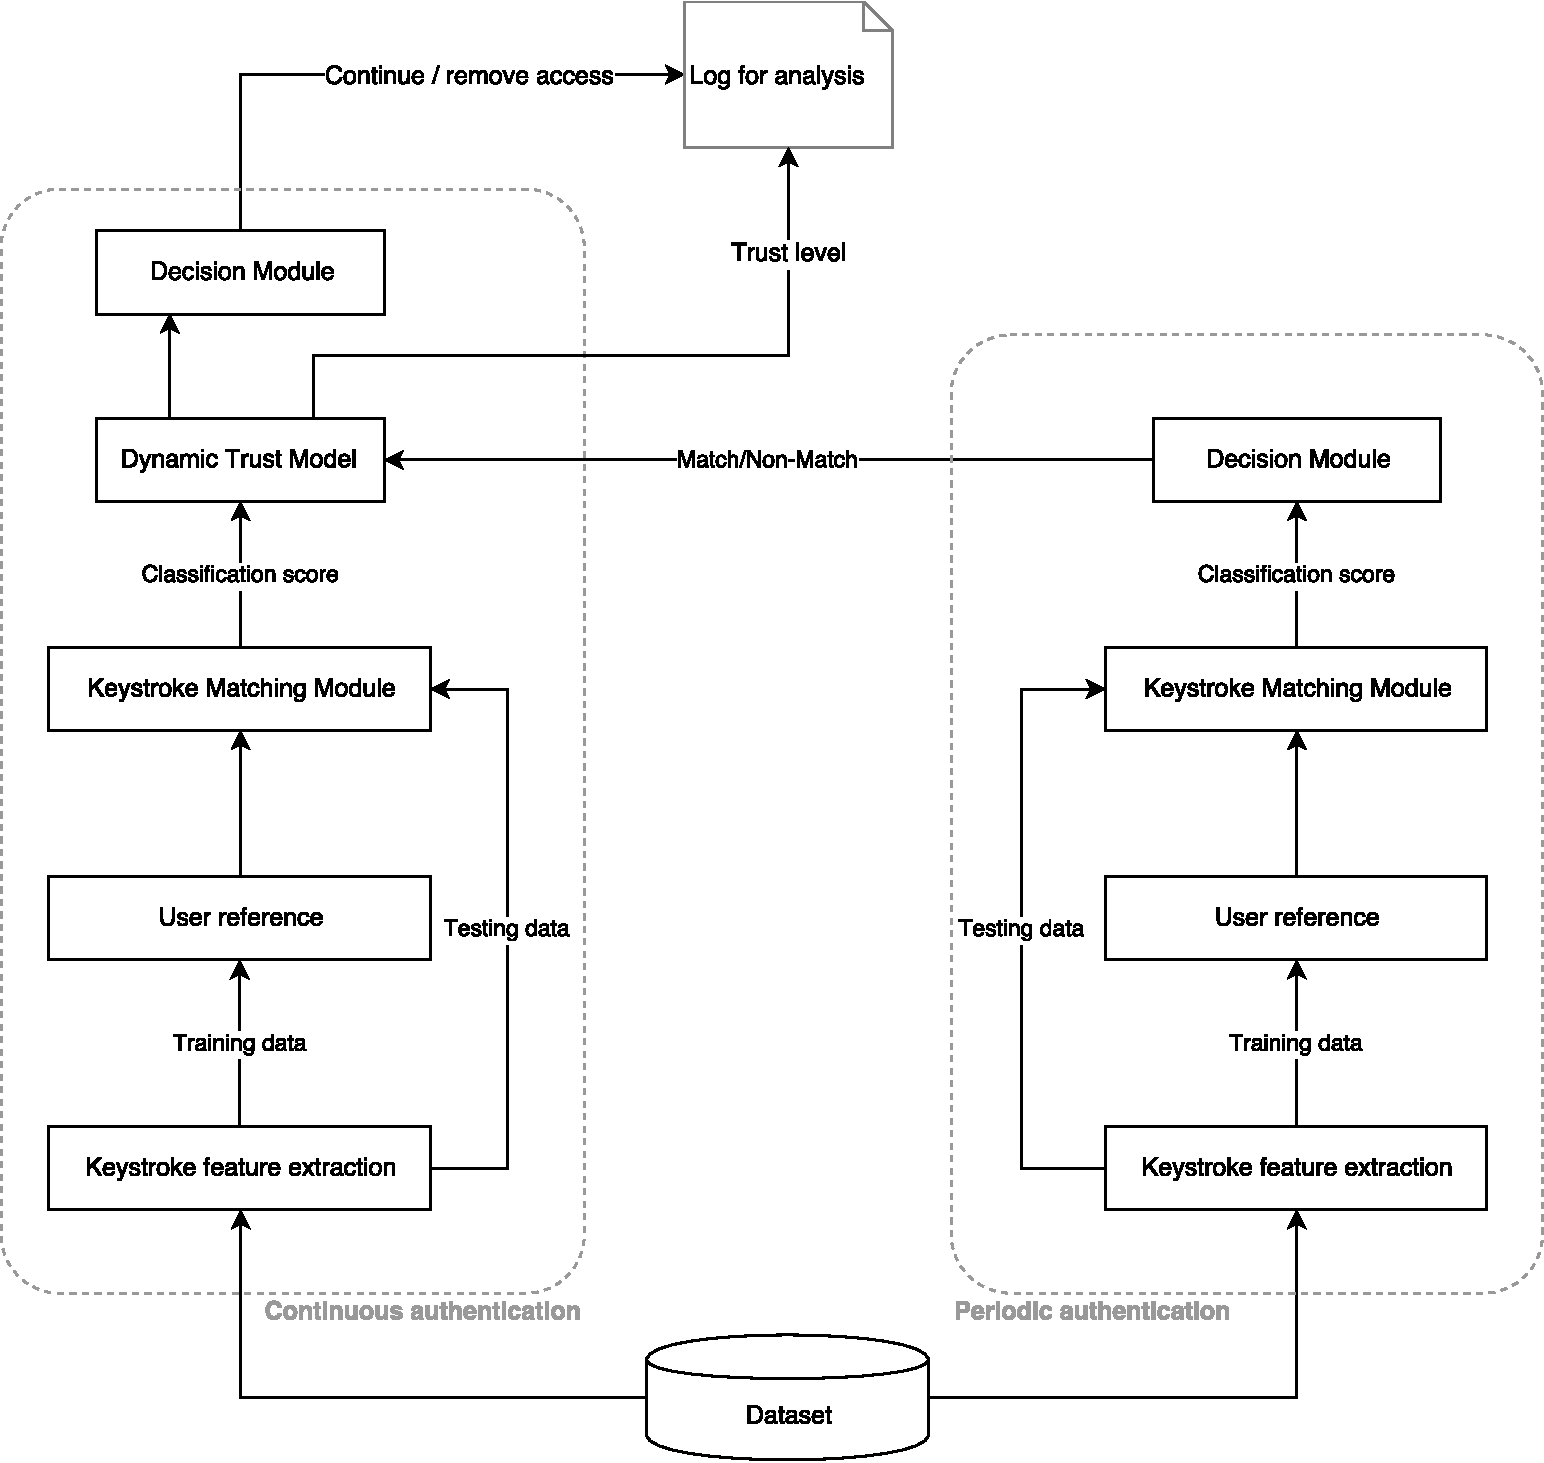
\includegraphics[width=0.8\textwidth]{system-diagram.pdf}
    \caption{Generalized diagram of how our systems may cooperate and produce data for analysis.}
    \label{fig:system-diagram}
\end{figure}

%Feature extraction
    %Features for CA system: single keys and digraphs
    %Features for PA system: could use the same, or base our choice on other literature

%
    
%

%

%Mention how the PA system may interact with the trust model OR make its own decision.

\section{Analysis}
Our main research question revolves around finding out if the performance of the original CA system can be improved by incorporating periodic authentication.
For this we will perform a \textit{quantitative} analysis \cite{leedy_ormrod_2013}.
More specifically, we can test the performance of the combined system by means of a leave-one-out cross validation test, which Mondal also did in his experiment.
The dataset includes 53 users, which means that for every genuine user we can test the performance using 52 imposters.
Performing these test will produce the necessary data for us to calculate the system's ANIA and ANGA values, as well as the number of undetected imposters.
During analysis, we will be able to adjust different variables to see its direct impact on performance, and tweak the system accordingly.
When doing so, we must avoid \textit{overfitting} our system to the specific dataset we are using.

For example, if decisions from the PA system are to be used as input to the Dynamic Trust Model, finding the optimal \textit{impact values} will be of great interest.
In such a case, the impact value would be how much the trust level would drop per periodic non-match, or how much it would increase per periodic match.
These two impact values may also be asymmetrical, i.e. periodic non-matches could decrease the trust level more than periodic matches would increase it.
There is clearly a large number of possible combinations of impact values, and we would naturally want to know which combination would give the best performance.
Optimizing these values using a relatively small subset of the users before applying them to the entire dataset could help us avoid a situation where performance of our system is significantly better on our dataset than on other unconstrained datasets.

We are also interested in keeping computational costs as low as possible, as seen in \textit{research sub-question 2}.
For this, we would like to analyze the processing time used per authentication.
Since we are incorporating PA into an existing CA system, the focus will be on minimizing the computational costs introduced by PA as opposed to decreasing the computational cost of the CA system.



%Leave one out

%NOTE: HUSK RESEARCH Q 1C!!!!!!!!!!!!!!!!!!!!!!!!!!!!!!!!!!!!!!!!!!!!!!!!!!!!!!!!!!!!


%This section is to include a description of the methods to be used,
%including references to literature describing the methods to be used
%(e.g. qualitative, quantitative, interviews, surveys,
%questionnaire,  model building etc.)
%For each of the research questions to be addressed,
%the chapter is to explain why the method is
%\begin{itemize}
%\item appropriate
%\item likely to provide the desired knowledge/information.
%\end{itemize}


\chapter{Milestones, deliverables and resources}
\label{chap:milestones}
%\begin{landscape}
%\begin{ganttchart}[
%hgrid,
%vgrid,
%x unit=2mm,
%time slot format=isodate
%]{2018-01-08}{2018-06-15}
%\gantttitlecalendar{month=name, week=2} \\
%\ganttbar{}{2018-01-14}{2018-01-17}
%\end{ganttchart}
%\end{landscape}


%\begin{landscape}
%\begin{ganttchart}[hgrid,
%                        vgrid,
%                        x unit=1.28mm,
%                        time slot format={isodate},
%                        ]{2018-01-08}{2018-06-15}
%           \gantttitlecalendar{year, month=name} \\
%           \ganttbar{Seminar}{2018-01-08}{2018-01-14} \\
%           \ganttbar{Review}{2018-01-15}{2018-01-21} \\
%           \ganttbar{Study CA}{2018-01-22}{2018-01-28} \\
%           \ganttbar{Feat. ext.}{2018-01-29}{2018-02-04} \\
%           \ganttbar{Train ref.}{2018-02-05}{2018-02-11} \\
%           \ganttbar{Probe proc.}{2018-02-12}{2018-02-18} \\
%           \ganttbar{Prep. alg.}{2018-02-19}{2018-02-25} \\
%           \ganttbar{Infl. CA}{2018-02-26}{2018-03-04} \\
%           \ganttbar{Perf. rep}{2018-03-05}{2018-03-11} \\
%           \ganttbar{Sim.}{2018-02-26}{2018-03-04} \\
%           \ganttbar{Analysis}{2018-02-26}{2018-03-04} \\
%           
%           %\ganttbar{Task 2}{2015-10}{2016-02} 
%      \end{ganttchart}
%\end{landscape}

%\begin{landscape}
%\begin{ganttchart}{1}{12}
%\gantttitle{2011}{12} \\
%\gantttitlelist{1,...,12}{1} \\
%\ganttgroup{Group 1}{1}{7} \\
%\ganttbar{Task 1}{1}{2} \\
%\ganttlinkedbar{Task 2}{3}{7} \ganttnewline
%\ganttmilestone{Milestone}{7} \ganttnewline
%\ganttbar{Final Task}{8}{12}
%\ganttlink{elem2}{elem3}
%\ganttlink{elem3}{elem4}
%\end{ganttchart}
%\end{landscape}
\section{Resources}
\label{sec:milestones-resources}
The only resource we will need is the dataset from Mondal's PhD thesis \cite{mondal}. The project's supervisor is already in possession of this dataset.
Access to the Biometrics Laboratory has been granted for the duration of the project.
No other resources are required, as the work will be done on personal computers.

\section{Preliminary table of contents}
\label{sec:milestones-toc}
Below is a representation of the planned structure of the MSc thesis.
This will help us plan what needs to be written throughout the project period.
It is also useful as a context reference for our thesis milestones described in \Cref{sec:milestones-deliverables-thesis}.
The table of context is temporary and certain parts may be changed, removed or added in the future.
\\\\
\noindent Title page\\
Abstract\\
Acknowledgements\\
Table of Contents\\
List of Tables\\
List of Figures\\
\\
\textbf{Introduction}\\
\indent Topic covered by the project\\
\indent Keywords\\
\indent Problem description\\
\indent Justification, motivation and benefits\\
\indent Research questions\\
\indent Planned contributions\\
\textbf{Background}\\
\indent Authentication\\
\indent Keystroke Dynamics\\
\textbf{Related work}\\
\indent Continuous authentication\\
\indent Periodic authentication\\
\textbf{Proposed system}\\
\indent Design\\
\indent Modules\\
\indent PA/CA interaction mechanism\\
\textbf{Analysis}\\
\indent Analysis of statistical approach\\
\indent Analysis of machine learning approach\\
\indent Discussion\\
\textbf{Future work}\\
\textbf{Conclusion}\\
\textbf{Bibliography}\\
\textbf{Appendixes}

\section{Deliverables}
\label{sec:milestones-deliverables}
The project has been split into incremental parts in order to help us keep track of progress during the project period.
Two main deliverables will be produced, with the first being the software implementations of the combined CA/PA system, and the second being the final MSc thesis including analysis results.
A number of milestones have been set for each of these deliverables, which can be seen in the following subsections.

\subsection{Software implementations}
\label{sec:milestones-deliverables-software}
Developing the software implementations of the CA/PA system is important for being able to answer our research question.
The implementations are needed for producing the data we are to analyze.
A total of four milestones has been set for this deliverable where the software will be presented to the supervisor:

\begin{enumerate}
    \item \textit{SA-1 implemented:} Having the implementation of the CA system's statistical approach ready is this deliverable's first milestone, as it sets up the next activity which is extending it with a PA system.
    \item \textit{SA-1 extended:} After having implemented the PA system and incorporated it into SA-1, the first analysis phase can be conducted.
    \item \textit{VP-3 implemented:} When the first analysis phase is over, the next milestone is having the CA machine learning approach implemented.
    \item \textit{VP-3 extended:} The last milestone of this deliverable is the machine learning approach of the CA system being extended with a PA system.
\end{enumerate}

\subsection{Master thesis}
\label{sec:milestones-deliverables-thesis}
We have also identified five milestones for the MSc thesis. 
Three other students have agreed to form a group where we will peer-review each others progress on the theses. 
Though it is subject to change, we have planned to perform the peer-reviews approximately once per month.
When the feedback is accounted for, a milestone is regarded as reached, and the current thesis progress is ready to be delivered to the supervisor.
Our thesis milestones are as follows:

\begin{enumerate}
    \item \textit{Thesis v.1:} Introduction, Background and Related work ready for delivery.
    \item \textit{Thesis v.2:} The combined CA/PA system's architecture is presented in the "Proposed system" chapter. Results from the first analysis documented.
    \item \textit{Thesis v.3:} Results from analysis 2 documented. Analysis chapter ready.
    \item \textit{Thesis v.4:} Future work, Conclusion, Abstract and Acknowledgements ready.
    \item \textit{Thesis v.5:} Final delivery. All feedback from supervisor is accounted for.
\end{enumerate}


\begin{figure}[h]
    \centering
    \rotatebox{90}{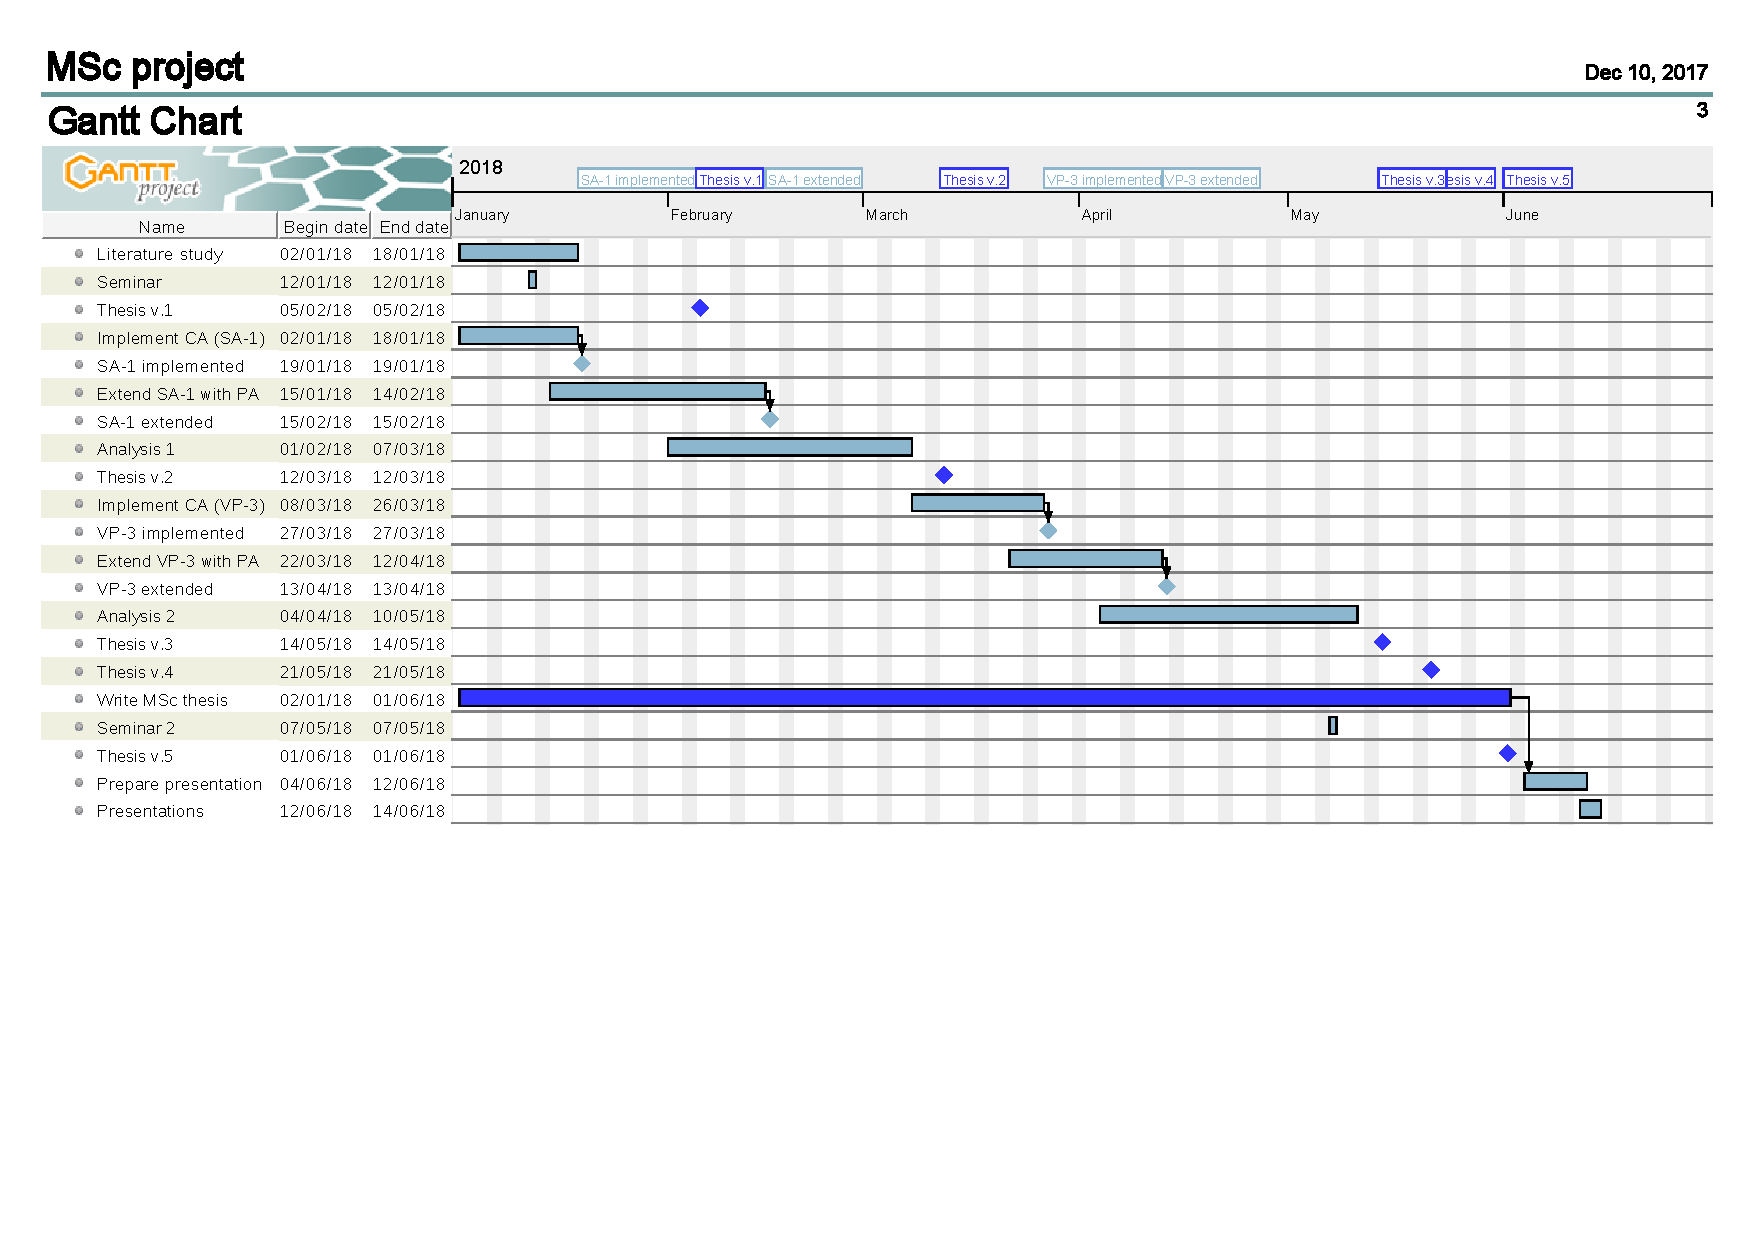
\includegraphics[width=1\textheight]{FinalGanttSplit.pdf}}
    \caption{Gantt chart of our planned progression throughout the project.}
    \label{fig:gantt}
\end{figure}

%\section{Implementing CA statistical approach}
%As mentioned in \Cref{sec:related-CA}, Mondal's \cite{mondal} dataset will be used in this project, allowing us to begin implementing his CA system at an early point of the project period. 

\section{Time management}
\label{sec:milestones-time}
We have made estimations of time needed for the planned activities in this project, and these can be found in \Cref{tab:hours}.
The estimations were made with 900 hours as a starting point, where approximately eight hours are spent on the project every monday through friday, including holidays.
If we begin to lag behind schedule, we can extend our working days by a number of hours and/or use weekends for catching up, increasing the total number of hours spent on the project.
Seminars are also not included, so the total hours will increase slightly depending on the length of the seminars.
A Gantt chart of our planned progression including milestones can be found in \Cref{fig:gantt}.

\begin{table}[h]
\centering
\resizebox{\textwidth}{!}{%
\begin{tabular}{lllll}
\hline
\textbf{Activity}             & \textbf{Description}                                                                                                                                                                                                                                                                                                                                    & \textbf{Starts} & \textbf{Ends} & \textbf{Hours} \\ \hline
\textit{Literature study}     & \begin{tabular}[c]{@{}l@{}}Review the most relevant CA and PA systems, \\ identify relevant work not yet covered.\end{tabular}                                                                                                                                                                                                                          & 02/01           & 18/01         & 50             \\ \hline
\textit{Implement CA (SA-1)}  & \begin{tabular}[c]{@{}l@{}}Implement SA-1 as described in \Cref{sec:related-CA}.\\We plan to implement all the software in MATLAB\\ due to its abundance of machine learning\\toolboxes, however this may change.\end{tabular}                                                                                                                                                                        & 02/01           & 18/01         & 25             \\ \hline
\textit{Extend SA-1 with PA}  & \begin{tabular}[c]{@{}l@{}}Implement PA system and incorporate it into the\\ CA system. As the exact methods to be used\\ in the PA system is yet to be decided, a larger \\ time frame is set for this activity to prepare for a\\ potentially complicated solution.\end{tabular}                                                                      & 15/01           & 14/02         & 150            \\ \hline
\textit{Analysis 1}           & \begin{tabular}[c]{@{}l@{}}Analyze the performance of the first \\ implementation of the combined system. \\ Perform cross validation tests, measure \\ ANIA/ANGA and undetected imposters. Also \\ measure the impact on processing speed. Make\\ changes to methods, variables and CA/PA \\ interaction to find the best performance.\end{tabular} & 01/02           & 07/03         & 125            \\ \hline
\textit{Implement CA (VP-3)}  & \begin{tabular}[c]{@{}l@{}}Develop the machine learning approach of \\ the CA system. Due to the complicated nature\\ of this approach, a large time frame is given.\end{tabular}                                                                                                                                                                       & 08/03           & 26/03         & 100            \\ \hline
\textit{Extend VP-3 with PA}  & \begin{tabular}[c]{@{}l@{}}Incorporate PA system into the machine learning\\ approach of the CA system. Depending on the PA\\ system, the interaction with the machine learning\\ approach may be hard to implement. If not, more\\ time is available for analysis.\end{tabular}                                                                        & 22/03           & 12/04         & 100            \\ \hline
\textit{Analysis 2}           & \begin{tabular}[c]{@{}l@{}}As Analysis 1. More time is given due to the \\ complexity of changing machine learning\\ variables.\end{tabular}                                                                                                                                                                                                            & 04/04           & 10/05         & 160            \\ \hline
\textit{Write MSc thesis}     & \begin{tabular}[c]{@{}l@{}}This is a continuous process beginning at the start\\ of the project period and lasting until the hand-in\\ date.\end{tabular}                                                                                                                                                                                               & 02/01           & 01/06         & 115            \\ \hline
\textit{Prepare presentation} & \begin{tabular}[c]{@{}l@{}}When the thesis is delivered, we have about a \\ week and a half for preparing the presentation. \\ There is a weekend of dead space here which \\ is likely to be used.\end{tabular}                                                                                                                                        & 04/06           & 12/06         & 75             \\ \hline
\\\textbf{Total hours}          & Excluding seminars. && & \textbf{900} \\ \\\hline
\end{tabular}
}
\caption{Estimated hours needed for activies.}
\label{tab:hours}
\end{table}


%The purpose of this chapter is to convince the reader that you know exactly what to do.
%This chapter gives a description of how the project is to be
%broken down into smaller parts and activities.
%\begin{enumerate}
%\item  What is it you have to do in order to obtain the desired knowledge?
%\item  What deliverables are to be produced (MSc thesis report, software,...)
%\item  When are the various deliverables going to be available?
%\end{enumerate}
%
%For each deliverable, identify 4 versions, having an
%'increasing' degree of completeness/quality.
%Students are strongly recommended to review each others drafts.
%For each version of a deliverable explain why and how this version is to
%be better/more complete.  E.g. v1.0: my first draft -
%chapter text includes 1/2 page summaries only.
%v.2.0: Like v1.0, but comments by NN(who? fellow student)
%has been incorporated. v3.0:....
%
%This section is to include a preliminary table of contents for the MSc thesis
%(only include 2 levels).
%
%For each of the activities identified, specify
%\begin{enumerate}
%\item  the time you need to complete each activity both calendar time and 'man-hours'.
%\item  hours needed by you
%\item  things you need to buy (consumables)
%\item  equipment, lab space or facilities you need access to
%\item  contributions from others (e.g. survey/interview participants) and how much each will have to contribute in terms of resources (probably time)
%\end{enumerate}
%At the beginning of this section, provide a 2-3 line summary of the
%resource requirements.  This is particularly useful if you have broken
%down the task into a lot of small tasks.
%
\chapter{Feasibility study}
We do not yet know whether the CA system's performance will be improved by the PA extension, as the goal of the project is to answer this question.
We do however have strong reason to believe that implementing a combined CA/PA system is possible.
This is due to the separate types of authentication systems already being implemented in literature, as discussed in \Cref{chap:related}.
We have also proposed a possible architecture of the combined system in \Cref{fig:system-diagram} in \Cref{sec:systemsetup} which further strengthens our belief of its feasibility.
A more pressing concern is therefore to discuss why results should be attainable within the limited time period.

It is not common practice for authors of PA (or CA) systems to state the amount of time used in their projects, with the exception of time spent on data collection.
It is therefore not easy to identify projects with similar time frames to ours.
What we can do is identify parts of our project that are expected to be difficult, and discuss how we can overcome problems associated with those parts.

We expect that implementing VP-3, extending it with a PA system and analyzing its performance will be one of the more challenging tasks of the project, due to having limited experience with machine learning and there being three different machine learning classifiers involved.
We mentioned in \Cref{sec:milestones-time} that we are likely to develop the software in MATLAB to benefit from its machine learning toolboxes, which can ease this issue.

Developing the PA system is also a task that could cause issues, depending on its complexity.
We have taken a precaution when planning the order of activities which can ensure that results still can be achieved even if we face major unexpected issues with either of the mentioned activities.
If we are unable to implement the machine learning approach, a compromise could be to reduce complexity by implementing a single machine learning algorithm as opposed to a multi-classifier fusion. 
In the worst case we can still fall back to the statistical approach and expand it, for example by incorporating another PA system and comparing how the two PA systems impact the CA system.
Choosing a different PA system is also a viable solution if we face issues incorporating PA into the CA statistical approach, as this issue would occur in the early phases of the project.


%Therefore split into two parts


%Matlab toolboxes, examples?
%

%An analysis of why it is likely that the desired
%results can be produced within the given time and
%resource bounds.  This may include a description of
%\begin{itemize}
%\item similar projects completed by others and their 'resource consumption',
%\item an attempt to answer parts of the research questions
%\item the 'difficult' elements of the work and an explanation of why/how these problems can be solved.  
%Alternatively you can explain an 'approximate' solution.
%\end{itemize}

\chapter{Risk analysis}
This chapter contains a risk analysis for the project period.
An attempt to estimate probability and impact of undesired events has been made, and the result can be seen in \autoref{tab:risk-analysis}.
The state of the risks have been visualized in \autoref{tab:initial-risk} and \autoref{tab:residual-risk}, before and after preventive or remedial actions have been considered.
The colors used in the risk analysis are explained in \autoref{tab:colour-legend}, and probability and impact classes are explained in \autoref{tab:probability-classes} and \autoref{tab:impact-classes}, respectively.

\begin{table}[H]
\scriptsize
\resizebox{\textwidth}{!}{%
\begin{tabular}{c| p{1.3cm}|p{1.5cm}|p{1.1cm}|p{2.37cm}|p{2.2cm}|p{1.7cm}|}
\hhline{~|------}
& \bf Identifier & Impl. CA & Illness & Impl. PA & Injury & Beh. sched.\\ \hhline{~|------|}
\bf & \bf Undesired event & Trouble implementing CA & Illness lasting a week or longer during project period & Trouble incorporating a PA system & Physical injury preventing progress & Falling far behind schedule\\ \hhline{~|------|} 
& \bf Probable Causes & Lack of understanding regarding original CA system; software bugs & Infection; other & Mathematical complexity; inexperience with Matlab & Severely injuring both hands or arms in a sport climbing accident & Too large workload; poor time management; burnout\\ \hhline{~|------|}
\multirow{3}{*}{\rotatebox{90}{\tiny INITIAL\,}} & \bf Probability & 3 & 2 & 4 & 1 & 3  \\ \hhline{~|------|}
& \bf Severity & 4 & 2 & 2 & 4 & 3 \\ \hhline{~|------|}
& \bf Risk Level & \cellcolor{red!50} & \cellcolor{green!50} & \cellcolor{yellow!50} & \cellcolor{yellow!50} & \cellcolor{yellow!50}\\ \hhline{~|------|}
& \bf Prevention/ Remediation& Ask for guidance from supervisor or the original author if necessary & None & Ask for guidance from supervisor; study Matlab implementations of machine learning and statistical models early in project period; prioritize another PA system & Only use highly experienced belayers during the project period; avoid climbing high-risk routes; request extension of deadline if injury occurs & Discuss which parts of the project can be omitted; extend working hours; socialize to prevent burnout\\ \hhline{~|------|}
\multirow{3}{*}{\rotatebox{90}{\tiny RESIDUAL\,}}& \bf Probability & 3 & 2 & 3 & 1 & 2\\ \hhline{~|------|}
& \bf Severity & 1 & 2 & 2 & 3 & 2\\ \hhline{~|------|}
& \bf Risk Level & \cellcolor{green!50} & \cellcolor{green!50} & \cellcolor{yellow!50} & \cellcolor{green!50} & \cellcolor{green!50}\\
\hhline{~|------|}

%add more rows as required
\end{tabular}
}
\caption{Risk analysis for project period}
\label{tab:risk-analysis}
\end{table}

\begin{table}[H]
\centering
\scriptsize
\resizebox{\textwidth}{!}{%
\begin{tabular}{|m{1.75cm}|m{1.75cm}|m{1.75cm}| m{1.75cm} |m{1.75cm}| m{1.75cm}|m{0cm}}
\hhline{|------|} \bf Probability/ Impact & \bf 1-Very unlikely & \bf 2-Unlikely & \bf 3-Possible & \bf 4-Likely & \bf 5-Very likely & \\[10pt]

\hhline{|------|} \bf 4-Catastrophic & \cellcolor{yellow!50} \centering Injury & \cellcolor{red!50}  & \cellcolor{red!50} \centering Impl. CA & \cellcolor{red!50} &\cellcolor{red!50} & \\ [10pt]

\hhline{|------|} \bf 3-Critical &\cellcolor{green!50} & \cellcolor{yellow!50} & \cellcolor{yellow!50} \centering Beh. sched. & \cellcolor{red!50} &\cellcolor{red!50} & \\ [10pt]

\hhline{|------|} \bf 2-Major & \cellcolor{green!50} & \cellcolor{green!50} \centering Illness & \cellcolor{yellow!50} &\cellcolor{yellow!50} \centering Impl. PA &\cellcolor{red!50}  & \\[10pt]

\hhline{|------|} \bf 1-Minor & \cellcolor{green!50} & \cellcolor{green!50} & \cellcolor{green!50} &\cellcolor{yellow!50} &\cellcolor{yellow!50} & \\ [10pt]
\hhline{|------|}
\end{tabular} 
}
\caption{Initial risk matrix}
\label{tab:initial-risk}
\end{table}

\begin{table}[H]
\centering
\scriptsize
\begin{tabular}{|m{1.75cm}|m{1.75cm}|m{1.75cm}| m{1.75cm} |m{1.75cm}| m{1.75cm}|m{0cm}}
\hhline{|------|} \bf Probability/ Impact & \bf 1-Very unlikely & \bf 2-Unlikely & \bf 3-Possible & \bf 4-Likely & \bf 5-Very likely & \\[10pt]

\hhline{|------|} \bf 4-Catastrophic & \cellcolor{yellow!50} & \cellcolor{red!50} & \cellcolor{red!50} & \cellcolor{red!50} &\cellcolor{red!50} & \\ [10pt]

\hhline{|------|} \bf 3-Critical &\cellcolor{green!50} \centering Injury & \cellcolor{yellow!50} & \cellcolor{yellow!50} & \cellcolor{red!50} &\cellcolor{red!50} & \\ [10pt]

\hhline{|------|} \bf 2-Major & \cellcolor{green!50} & \cellcolor{green!50} \centering Beh. sched.; Illness & \cellcolor{yellow!50} \centering Impl. PA &\cellcolor{yellow!50} &\cellcolor{red!50} & \\[10pt]

\hhline{|------|} \bf 1-Minor & \cellcolor{green!50} & \cellcolor{green!50} & \cellcolor{green!50} \centering Impl. CA &\cellcolor{yellow!50} &\cellcolor{yellow!50} & \\ [10pt]
\hhline{|------|}
\end{tabular} \\
\caption{Residual risk matrix}
\label{tab:residual-risk}
\end{table}

The analysis includes events with significant probability and impact.
As seen in tables 1-3, there are no residual risks with red risk level.
The event with a yellow residual risk level is Impl. PA.
While the impact of this event is not critical, a high probability remains.
Incorporating the PA system into the CA system is one of the main tasks of the master thesis, and a high probability of having trouble with this is only natural.
Therefore, trying to remediate this event any further is part of the project itself.

\begin{table}[H]
\centering
%\scriptsize
\begin{tabular}{|p{2cm}|p{10cm}|}
\hline \bf Colour & \bf Legend \\
\hline \cellcolor{red! 50} & Not acceptable - Risk reduction required \\ [10pt]
\hline \cellcolor{yellow! 50} & Acceptable to a some degree. Consider further risk reduction. \\[10pt]
\hline \cellcolor{green! 50} & Acceptable. \\ [10pt]
\hline
\end{tabular}
\caption{Risk matrix color legend}
\label{tab:colour-legend}
\end{table}

\begin{table}[H]
\centering
\begin{tabular}{ p{2cm} p{3cm} p{8cm}}
\hline \bf Rank & \bf Probability class & \bf Description \\
\hline 1 & Very unlikely & Below 5 \% chance of occurring \\
2 & Unlikely & Between 5 - 25 \% chance of occurring \\
3 & Possible & Between 25 - 75 \% chance of occurring \\
4 & Likely & Between 75 - 95 \% chance of occurring \\
5 & Very likely & Over 95\% chance of occurring \\

\hline

\end{tabular}
\caption{Probability classes legend}
\label{tab:probability-classes}
\end{table}

%Severity Classes Legend
\begin{table}[H]
\centering
\begin{tabular}{ p{2cm} p{3cm} p{8cm}}
\hline \bf Rank & \bf Severity class & \bf Description \\

\hline 4 & Catastrophic & Events lead to complete project failure. \\
3 & Critical & Events lead to very large set-backs, with significant negative impact on end result.\\
2 & Major & Events lead to important parts of the project being negatively affected. \\
1 & Minor & Events lead to smaller parts of minimal importance being negatively affected or omitted.\\
\hline
\end{tabular}
\caption{Impact classes legend}
\label{tab:impact-classes}
\end{table}


%\begin{itemize}
%\item What can possibly go wrong when you do your project?
%\item How do you intend to reduce impact of/solve these problems?
%\end{itemize}



\chapter{Ethical and legal considerations}
Doing research in the biometrics field brings ethical problems and legal considerations, as it often involves collecting highly sensitive information from volunteers contributing to the project.
This is especially true for unconstrained free-text keystroke dynamics, as the data collected involves not only measurements of the biometric trait, but also information that can be analyzed to uncover the semantics and context of what the participants typed on their private computers. 

The dataset to be used \cite{mondal} was collected from consenting participants following the guidelines of the \textit{Norwegian Data Protection Authority} in order to comply with the Personal Data Act of 2000\footnote{https://www.datatilsynet.no/en/regulations-and-tools/regulations-and-decisions/norwegian-privacy-law/personal-data-act/}.
Our handling of the data will also be in accordance with this act, and we will also follow guidelines to ensure compliance.
The supervisor possesses the dataset as stated in \Cref{sec:milestones-resources}, and it can be used for research at NTNU.

The data was collected using a logging tool which automatically censored passwords when logging the keystrokes. 
This is one measure that decreases the amount of highly sensitive information collected to a certain degree.
Still, some password fields may not have been detected by the tool, resulting in keystrokes involved in passwords being recorded without censoring. 
Even if all passwords were censored, a very large amount of keystroke data was recorded, and some forms of sensitive information is bound to be present in the database.

Our analysis will be automated, and we will not visually inspect raw keystroke samples unless it is absolutely necessary for project progression.
If we do access raw samples, we will refrain from analyzing the semantics of the data, i.e. what was being written.
No sensitive information derived from raw samples will be shared with anyone who are not members of the project (being the author and the supervisor), and it will not be presented in the MSc thesis.

Under no circumstances will access to the dataset or a subset of its data be given to any third party.
When the project period is over, all data from the dataset will be removed from the project members' devices, and stored on a secure university server for future research purposes.


%The purpose of this chapter is to convince the
%reader and your self that your project activities are
%\begin{itemize}
%\item legal
%\item ethical, e.g. don't use/distribute/collect etc. data in such a way that individuals may suffer.
%\end{itemize}
%For example, if you are planning to do reverse engineering activities, surveys, PENTESTING- (both technical and based on social engineering techniques) you need to be particularly careful and check with the appropriate experts and authorities if the activity is permitted.  An explanation of why your project is both legal and ethical should be given in this chapter.
%
%If you need permission (e.g. because you will be collecting or processing privacy related information), 
%you should  include the appropriate applications/application forms and ensure that these applications 
%are submitted well before you need the permission.

%9.  Bibliography (1-3 pages)

%\chapter{The bibliography}
%References/bibliography
%Reference to other peoples work MUST include:
%\begin{itemize}
%\item Name of author(s)  or name of responsible organization (if the document does not have a named author.
%\item Title of document.
%\item Where published.
%\item Year of publication.
%\end{itemize}
%
%There are many different types of documents (article, book etc.).
%In many cases, the required/optional fields may differ.
%See e.g. the BibTeX entry of wikipedia (\url{http://en.wikipedia.org/wiki/BibTeX}).
%The bibliography file 
%\verb+imt4441.bib+ 
%contains an example.
%
%NOTE: A url on its own is no good!
%It must be possible to locate the reference even if a link goes dead!
%
%\appendix
%\chapter{Known problems with MikTeX and TeXnicCenter}
%\section{Hig logo xor url's}
%\paragraph{Problem}
%Using MikTeX (version 2.6) in combination with TeXnicCenter you may experience the following problems:
%
%You have to choose between being able to get the HIG logo on the front page (Use the TeXnic translation LaTeX => ps => pdf)  and getting visible url's (use the LaTeX => PDF translation option).
%
%\paragraph{Possible solution 1}
%use \verb+\usepackage[dvips]{graphicx}+ in combination with TeXnicCenter translation LaTeX => PS, and use Adobe distiller to convert from PS to PDF.  This should give both logo and URL (but no line breaks in URL's).
%
%\paragraph{Possible solution 2}
%Use \verb+epstopdf.exe+ to convert \verb+higlogo.eps+ to \verb+higlogo.pdf+.
%Modify the file \verb+gucmasterthesis.cls+ to include \verb+higlogo.pdf+ instead of \verb+higlogo+.
%Select the TeXnicCenter translation \verb+LaTeX => PDF+.
%
%
%\section{\LaTeX/AFPL Ghostscript crashes}
%\paragraph{Problem}
%The build window prints out operand stack, execution and dictionary stack before concluding with the message 
%'\verb+Unrecoverable error, exit code 1+'.
%\paragraph{Possible solution}
%Use the TeXnicCenter translation 'LaTeX => PDF'.
%
%\chapter{Project description evaluation criteria}


\bibliographystyle{plain}
%\bibliographystyle{gucmasterthesis}
\bibliography{imt4441}



\end{document}





%IEEE computer society keywords
%http://www.computer.org/portal/site/ieeecs/menuitem.c5efb9b8ade9096b8a9ca0108bcd45f3/index.jsp?&pName=ieeecs_level1&path=ieeecs/publications/author/keywords&file=ACMtaxonomy.xml&xsl=generic.xsl&
